\documentclass{article}

\usepackage{amsthm, amsfonts, amsmath, amssymb}
\usepackage{graphicx}
\usepackage{fullpage}
\usepackage{float}

\usepackage{xcolor}
\definecolor{commentsColor}{rgb}{0.497495, 0.497587, 0.497464}
\definecolor{keywordsColor}{rgb}{0.000000, 0.000000, 0.635294}
\definecolor{stringColor}{rgb}{0.558215, 0.000000, 0.135316}
\usepackage{listings}
\lstset{ %
	backgroundcolor=\color{white},   				% choose the background color; you must add \usepackage{color} or \usepackage{xcolor}
	basicstyle=\footnotesize\ttfamily,				% the size of the fonts that are used for the code
	breakatwhitespace=false,         				% sets if automatic breaks should only happen at whitespace
	breaklines=true,                 				% sets automatic line breaking
	captionpos=b,                    				% sets the caption-position to bottom
	commentstyle=\color{commentsColor}\textit,		% comment style
	frame=tb,	                   	   				% adds a frame around the code
	keywordstyle=\color{keywordsColor}\bfseries,	% keyword style
	language=Python,                 				% the language of the code (can be overrided per snippet)
	otherkeywords={*,...},           				% if you want to add more keywords to the set
	rulecolor=\color{black},         				% if not set, the frame-color may be changed on line-breaks within not-black text (e.g. comments (green here))
	stringstyle=\color{stringColor}, 				% string literal style
	title=\lstname,                  				% show the filename of files included with \lstinputlisting; also try caption instead of title
	columns=fixed                   				% Using fixed column width (for e.g. nice alignment)
}

\usepackage{hyperref}

\newtheorem{lemma}{Lemma}
\newtheorem{theorem}{Theorem}
\newtheorem{corollary}{Corollary}
\newtheorem{conjecture}{Conjecture}
\newtheorem{definition}{Definition}

\setlength{\parindent}{0em}

\renewcommand{\O}{\mathcal{O}}
\newcommand{\N}{\mathbb{N}}
\newcommand{\xor}{\oplus}

\begin{document}
	\title{The Rank Deficiency of Certain Sized \textit{Lights Out} Boards}
	\author{William Boyles}
	\date{\today}
	\maketitle
	
	\section{Intro Conjectures}
	Let $f(n,x)$ be the Chebyshev polynomial over $GF(2)$ that we defined previously.
	Recall that the rank deficiency of an $n \times n$ \textit{Lights Out} board, $d(n)$, is the degree of $\gcd(f(n,x), f(n,x+1))$.
	Let $g: \N \to \N$ where $g(k) = 2^{k+1} + 2^{k-1} - 1$.

	\begin{conjecture}
		\label{conj1}
		Let $k \in \N$.
		Then
		\begin{equation*}
			f(g(k), x) = x^{2^{k-1}-1}\left(x^{2^{k+1}}+x^{2^k}+1\right).
		\end{equation*}
	\end{conjecture}

	\begin{conjecture}
		\label{conj2}
		Let $k \in \N$.
		Then
		\begin{equation*}
			f(g(k), x+1) = \left(x^{2^{k+1}}+x^{2^k}+1\right)\left(x^{2^{k-1}-1}+\dots+1\right).
		\end{equation*}
	\end{conjecture}
	
	\section{Main Result}
	The following relies on \ref{conj1} and \ref{conj2} being true.
	\begin{theorem}
		Let $k \in \N$.
		Then
		\begin{equation*}
			\gcd\left(f(g(k),x),f(g(k),x+1)\right) = x^{2^{k+1}} + x^{2^k} + 1.
		\end{equation*}
	\end{theorem}
	\begin{proof}
		We can see from conjectures 1 and 2 that the desired gcd is a common factor of both polynomials.
		So, we just need to show that over $GF(2)$ that the remaining factors of both polynomials have no common factors.
		This result is easily verified by a computer.
		
		\begin{figure}[H]
			\centering
			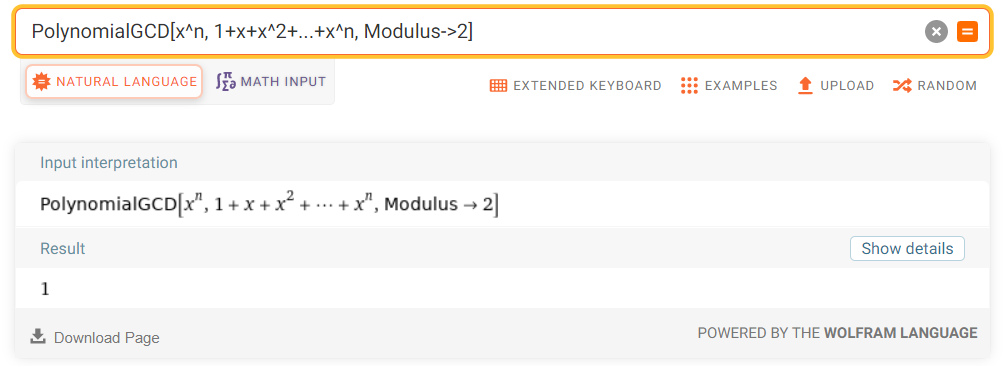
\includegraphics[width=.8\textwidth]{wolfram_result.png}
			\caption{\href{https://www.wolframalpha.com/input/?i=PolynomialGCD\%5Bx\%5En\%2C+1\%2Bx\%2Bx\%5E2\%2B...\%2Bx\%5En\%2C+Modulus-\%3E2\%5D}{Wolfram|Alpha: PolynomialGCD[$x^n, 1+x+x^2+...+x^n$, Modulus$\to$2]}}
		\end{figure}
	\end{proof}

	\begin{corollary}
		A \textit{Lights Out} board of size $g(k) \times g(k)$ will have nullity $2^{k+1}$.
	\end{corollary}
	
	\section{Concluding Conjectures}
	\begin{conjecture}
		\label{conj3}
		Let $h: \N \to \N$ where
		\begin{equation*}
			h(n) = \max \{g(m) \mid m \in \N, g(m) \leq n\}.
		\end{equation*}
		Then for all $n \in \N$,
		\begin{equation*}
			\max \{d(m) \mid 1 \leq m \leq n\} = d(h(n)).
		\end{equation*}
	\end{conjecture}
	
	\begin{corollary}
		$d(n) = n$ only for $n=4$.
		Otherwise, $d(n) < n$.
	\end{corollary}
	\begin{proof}
		Observe that $d(1) = d(2) = d(3) = 0$, and $d(g(1)) = d(4) = 4$. \\
		
		Assume for contradiction that there exists some $n > 4$ such that $d(n) \geq n$.
		
		Notice that for $k > 1$,
		\begin{equation*}
			d(g(k)) = 2^{k+1} < g(k) = 2^{k+1} + 2^{k-1} - 1.
		\end{equation*}
		So,
		\begin{equation*}
			d(h(n)) < h(n) \leq n = d(n).
		\end{equation*}
	
		However,
		\begin{equation*}
			\max \{d(m) \mid 1 \leq m \leq n\} = d(n) > d(h(n)),
		\end{equation*}
		which contradicts conjecture \ref{conj3}.
	\end{proof}
\end{document}